\documentclass{beamer}
%
% Choose how your presentation looks.
%
% For more themes, color themes and font themes, see:
% http://deic.uab.es/~iblanes/beamer_gallery/index_by_theme.html
%
\mode<presentation>
{
  \usetheme{default}      % or try Darmstadt, Madrid, Warsaw, ...
  \usecolortheme{default} % or try albatross, beaver, crane, ...
  \usefonttheme{default}  % or try serif, structurebold, ...
  \setbeamertemplate{navigation symbols}{}
  \setbeamertemplate{caption}[numbered]
}

\usepackage[english]{babel}
\usepackage[utf8x]{inputenc}

\usepackage{amstext}
%\usepackage{coloremoji}
\usepackage{layout}
\usepackage{multirow}

\usepackage{graphicx}
\graphicspath{ {figs/} }

\setbeameroption{hide notes}
\setbeamertemplate{note page}[plain]
\usepackage{listings}
\usepackage{datetime}
\usepackage{url}

% specifications for presenter mode
%\beamerdefaultoverlayspecification{<+->}
%\setbeamercovered{transparent}

% math shorthand
\usepackage{bm}
\usepackage{amsmath}
\usepackage{mathtools}
\newcommand{\R}{\mathbb{R}}
\newcommand{\D}{\mathcal{D}}
\newcommand{\E}{\mathbb{E}}
\newcommand{\F}{\mathcal{F}}
\newcommand{\X}{\mathcal{X}}
\newcommand{\lik}{\mathcal{L}}
\DeclarePairedDelimiterX{\infdivx}[2]{(}{)}{%
  #1\;\delimsize\|\;#2%
}
\newcommand{\infdiv}{D\infdivx}
\DeclarePairedDelimiter{\norm}{\lVert}{\rVert}
\DeclareMathOperator*{\argmin}{arg\,min}
\DeclareMathOperator*{\argmax}{arg\,max}

% Bibliography
\usepackage{natbib}
\bibpunct{(}{)}{,}{a}{}{;}
\usepackage{bibentry}

%\nobibliography*
\title[zinbwave-droplasso]{Differential Expression Analysis Techniques for
  Single-Cell RNA-seq Experiments}
\subtitle{\vspace*{0.5em} \scriptsize for the Computational Biology Doctoral
  Seminar (CMPBIO 293),\\ organized by N.~Yosef \& T.~Ashuach, Spring 2018, UC
  Berkeley}
\author{Kevin Benac and Nima Hejazi}
\institute{Group in Biostatistics,\\ University of California, Berkeley}
\date{11 April 2018}

%%%%%%%%%%%%%%%%%%%%%%%%%%%%%%%%%%%%%%%%%%%%%%%%%%%%%%%%%%%%%%%%%%%%%%%%%%%%%%%%

%\setcounter{tocdepth}[2]
\AtBeginSubsection[]{
\begin{frame}{Outline}
\tableofcontents[currentsection,currentsubsection]
\end{frame}
}

%%%%%%%%%%%%%%%%%%%%%%%%%%%%%%%%%%%%%%%%%%%%%%%%%%%%%%%%%%%%%%%%%%%%%%%%%%%%%%%%

\begin{document}

\begin{frame}
  \titlepage
\end{frame}

%%%%%%%%%%%%%%%%%%%%%%%%%%%%%%%%%%%%%%%%%%%%%%%%%%%%%%%%%%%%%%%%%%%%%%%%%%%%%%%%
\section{Introduction}
\subsection{Data}
%%%%%%%%%%%%%%%%%%%%%%%%%%%%%%%%%%%%%%%%%%%%%%%%%%%%%%%%%%%%%%%%%%%%%%%%%%%%%%%%

\begin{frame}{The Data: Single-Cell RNA-seq}
\begin{itemize}
  \itemsep10pt
  \item scRNA-seq fast growing approach to measure the genome-wide transcriptome
    of many individual cells in parallel (Kolodziejczyk et al., 2015).
  \item Major advance compared to standard “bulk” RNA sequencing to investigate
    complex heterogeneous tissues,
  \item Access to cell-to-cell variability: better accuracy.
\end{itemize}

\end{frame}

%%%%%%%%%%%%%%%%%%%%%%%%%%%%%%%%%%%%%%%%%%%%%%%%%%%%%%%%%%%%%%%%%%%%%%%%%%%%%%%%

\begin{frame}{The Data: Single-Cell RNA-seq}

%No free lunch thm
\begin{itemize}
  \itemsep10pt
  \item However, analysis of single-cell RNA-seq data is challenging.
  \item In one cell, only a tiny amount of RNA is present and large fraction of
    polyadenylated RNA can be stochastically lost during sample preparation
    steps (cell lysis, reverse transcription or amplification). \\
    $\Longrightarrow$ Many genes fail to be detected although they are
    expressed!
  \item In practice, not uncommon to end up with a matrix of read counts where
    about 80\% of the coefficients are zeros.
  \item This zeros are called \textit{dropouts}.
\end{itemize}

\end{frame}

%%%%%%%%%%%%%%%%%%%%%%%%%%%%%%%%%%%%%%%%%%%%%%%%%%%%%%%%%%%%%%%%%%%%%%%%%%%%%%%%

\begin{frame}{The Data: Single-Cell RNA-seq}

\begin{table}[ht]
\centering
\begin{tabular}{rrrrrrrrrrr}
  \hline
 & Cell1 & Cell 2 & Cell 3 & Cell 4 & Cell 5 & Cell 6 & Cell 7  \\
  \hline
  Xkr4 & 0 & 0 & 0 & 14 & 0 & 0 & 0  \\
  Syt11 & 1 & 9 & 2 & 2 & 0 & 0 & 0  \\
  Cpe & 0 & 0 & 16 & 0 & 0 & 0 & 0  \\
  Rp1 & 0 & 0 & 0 & 0 & 0 & 0 & 0  \\
  Gm73 & 0 & 0 & 0 & 0 & 0 & 0 & 0  \\
  Gm79 & 0 & 0 & 0 & 0 & 0 & 0 & 0  \\
  Mpl15 & 8 & 8 & 6 & 1 & 0 & 0 & 0  \\
  Gm61 & 0 & 0 & 0 & 0 & 0 & 3 & 0 \\
  Lypla1 & 1 & 23 & 266 & 1 & 0 & 1 & 0 \\
  Tcea1 & 63 & 101 & 18 & 29 & 2 & 34 & 0 \\
   \hline
\end{tabular}
\end{table}

\end{frame}

\begin{frame}{The Data: Single-Cell RNA-seq}

\begin{itemize}
  \itemsep10pt
  \item Raises modelling and computational issues.
  \item Need to detect a signal when most of the values are zeros only because
    they are missing.
  \item Traditional methods used for bulk RNA-seq data might not be sensible
    anymore.
\end{itemize}

\end{frame}

%%%%%%%%%%%%%%%%%%%%%%%%%%%%%%%%%%%%%%%%%%%%%%%%%%%%%%%%%%%%%%%%%%%%%%%%%%%%%%%%
\subsection{Objective}
%%%%%%%%%%%%%%%%%%%%%%%%%%%%%%%%%%%%%%%%%%%%%%%%%%%%%%%%%%%%%%%%%%%%%%%%%%%%%%%%

\begin{frame}{The Objective: Differential Expression}

\begin{itemize}
  \itemsep12pt
  \item Why ``differential''? The goal is to find a subset of relevant
    biomarkers with respect to a particular condition of interest (e.g.,
    disease, tissue of origin).
  \item Many experimental settings seek to isolate a subset of biomarkers from
    the full (larger) assayed set in order to identify biological patterns and
    better inform future biological experiments.
  \item Since experimental costs are high and modern biotechnologies allow
    numerous biological targets (e.g., genes) to be assayed, the result is a
    very high-dimensional statistical problem.
\end{itemize}

\end{frame}

%%%%%%%%%%%%%%%%%%%%%%%%%%%%%%%%%%%%%%%%%%%%%%%%%%%%%%%%%%%%%%%%%%%%%%%%%%%%%%%%

\begin{frame}{The Objective: Differential Expression}

\begin{itemize}
  \itemsep12pt
  \item Regularized Linear Models:
    \[
      \min_{w \in \R^d} \left\{ \frac{1}{n} \sum_{i = 1}^n \lik(w, x_i, y_i) +
        \lambda \Omega(w) \right\}
    \]
  \item Lasso for continuous outcomes (squared-error loss):
    \[
      \min_{w \in \R^d} \left\{ \frac{1}{n} \sum_{i = 1}^n \left(y_i - \sum_{j =
        1}^d w_j x_{i,j} \right)^2 + \lambda \sum_{j = 1}^d \lvert w_j \rvert
        \right\}
    \]
\end{itemize}

\end{frame}

%%%%%%%%%%%%%%%%%%%%%%%%%%%%%%%%%%%%%%%%%%%%%%%%%%%%%%%%%%%%%%%%%%%%%%%%%%%%%%%%
\section{Methodology}
\subsection{ZINB-WaVE}
%%%%%%%%%%%%%%%%%%%%%%%%%%%%%%%%%%%%%%%%%%%%%%%%%%%%%%%%%%%%%%%%%%%%%%%%%%%%%%%%

\begin{frame}{ZINB-WaVE}

\begin{itemize}
  \itemsep10pt
  \item Method that leads to low-dimensional representations of the data the
    same way PCA or tSNE does. \pause
  \item However accounts for zero inflation (dropouts), over-dispersion, and the
    count nature of the data.
  \item No need for normalization.
\end{itemize}

\end{frame}
%%%%%%%%%%%%%%%%%%%%%%%%%%%%%%%%%%%%%%%%%%%%%%%%%%%%%%%%%%%%%%%%%%%%%%%%%%%%%%%%




\begin{frame}{ZINB-WaVE}
Mathematical set-up:
\begin{itemize}
  \itemsep10pt
  \item $n$ samples (single-cells),
  \item $J$ genes,
  \item $Y_{ij}$ read counts for gene $j$ in cell $i$, $1\leq \ldots \leq n,
    \quad 1\leq j \leq J.$,
  \item $\pi_{ij}$: probability of dropout,
  \item $\mu_{ij}$: mean expression level.
\end{itemize}

\end{frame}

%%%%%%%%%%%%%%%%%%%%%%%%%%%%%%%%%%%%%%%%%%%%%%%%%%%%%%%%%%%%%%%%%%%%%%%%%%%%%%%%

\begin{frame}{ZINB-WaVE}
\begin{figure}
  \centering
      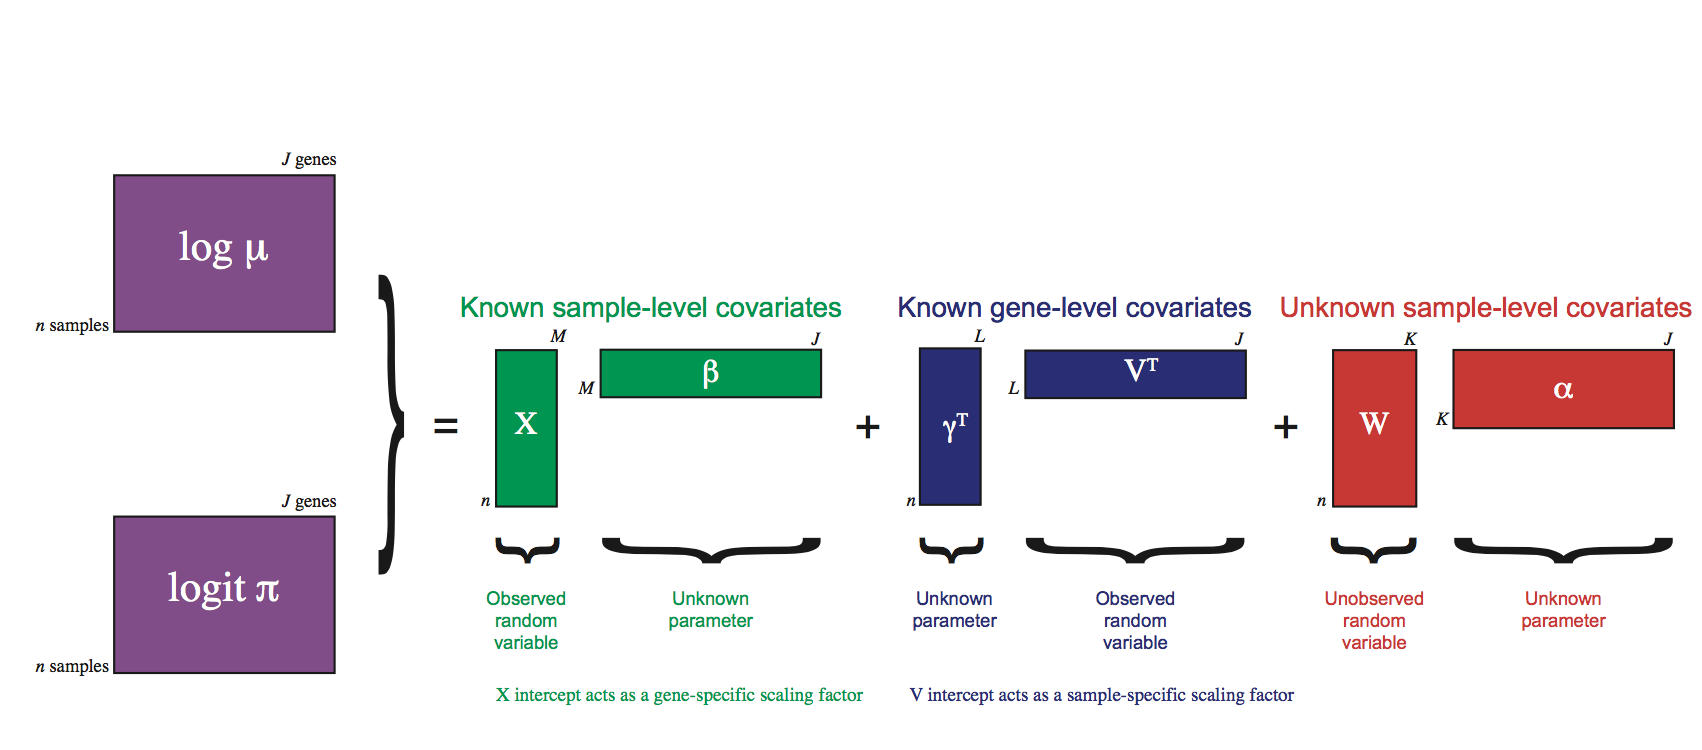
\includegraphics[height=0.5\textheight]{zinbwave}
      \caption{The ZINB-WaVE model}
\end{figure}
\end{frame}

%%%%%%%%%%%%%%%%%%%%%%%%%%%%%%%%%%%%%%%%%%%%%%%%%%%%%%%%%%%%%%%%%%%%%%%%%%%%%%%%

\begin{frame}{ZINB-WaVE}
\begin{itemize}
  \itemsep10pt
  \item ZINB-WaVE mainly used for normalization and dimensionality reduction but
    can also be used for DE analysis.
  \item Compute weights from the estimated $\pi$ using Bayes formula.
  \item If the observed counts are positive, $w = 1$, otherwise, $0<w<1$.
  \item The higher $\pi$, the lower $w$
\end{itemize}
\end{frame}

%%%%%%%%%%%%%%%%%%%%%%%%%%%%%%%%%%%%%%%%%%%%%%%%%%%%%%%%%%%%%%%%%%%%%%%%%%%%%%%%

\begin{frame}{ZINB-WaVE}

\begin{itemize}
  \itemsep10pt
  \item Once we have the weights, fit a weighted negative binomial generalized
    linear model using the ZINB-WaVE weights.
  \item End-up with a matrix of fitted values.
  \item Not sparse anymore, look more like bulk RNA-seq data.\\
    $\Longrightarrow$ We can use classical tools for differential expression
    analysis (e.g.~edgeR, DESeq2, limma-voom in R/Bioconductor).
\end{itemize}

\end{frame}

%%%%%%%%%%%%%%%%%%%%%%%%%%%%%%%%%%%%%%%%%%%%%%%%%%%%%%%%%%%%%%%%%%%%%%%%%%%%%%%%
%%%%%%%%%%%%%%%%%%%%%%%%%%%%%%%%%%%%%%%%%%%%%%%%%%%%%%%%%%%%%%%%%%%%%%%%%%%%%%%%
\subsection{DropLasso}
%%%%%%%%%%%%%%%%%%%%%%%%%%%%%%%%%%%%%%%%%%%%%%%%%%%%%%%%%%%%%%%%%%%%%%%%%%%%%%%%

\begin{frame}{DropLasso}

\begin{itemize}
  \itemsep12pt
  \item Consider the following data structure:
    \begin{itemize}
      \itemsep10pt
      \item $x_i \in \mathbb{R}^d$ --- design matrix of scRNA-seq counts
      \item $y_i \in \mathbb{R}$ --- cell-level outcome of interest (e.g.,
        tissue of origin)
      \item $\delta_i \in \{0, 1\}^d$ s.t.~$\delta_i \sim Bern(p)^d$ --- random
        dropout mask
      \item $\delta \odot x \in \mathbb{R}^d$ --- corrupted pattern for
        scRNA-seq dropout
      \item $\text{P}(\delta_i = 1) = \text{p}$ --- probability of \textit{not}
        being censored by dropout
    \end{itemize}
  \item The DropLasso procedure seeks to identify differentially expressed genes
    based on cell-level differences while accounting for the dropout noise that
    masks scRNA data.
\end{itemize}

\end{frame}

%%%%%%%%%%%%%%%%%%%%%%%%%%%%%%%%%%%%%%%%%%%%%%%%%%%%%%%%%%%%%%%%%%%%%%%%%%%%%%%%

\begin{frame}{DropLasso}

\begin{itemize}
  \itemsep12pt
  \item Introducing dropout ($\delta_i \sim Bern(p)^d$):
    \[
      \min_{w \in \R^d} \left\{ \frac{1}{n} \sum_{i = 1}^n \E_{\delta_i}
        \lik \left(w, \delta_i \odot \frac{x_i}{p}, y_i \right) + \lambda
        \lVert w \rVert_1 \right\}
    \]
  \item Independence from $p$ in expectation:
    \[
      \begin{aligned}
      \E_{\delta_i} \sum_{j = 1}^{d} w_j \left( \delta_i \odot \frac{x_i}{p}
      \right)_j =& \sum_{j = 1}^d \E_{\delta_i} w_j \delta_{i,j}
      \frac{x_{i,j}}{p} \\ =& \sum_{j = 1}^d w_j x_{i,j}
      \end{aligned}
    \]
\end{itemize}

\end{frame}

%%%%%%%%%%%%%%%%%%%%%%%%%%%%%%%%%%%%%%%%%%%%%%%%%%%%%%%%%%%%%%%%%%%%%%%%%%%%%%%%

\begin{frame}{DropLasso}

\begin{itemize}
  \itemsep12pt
  \item Introducing the dropout term $\delta$ amounts to censoring the observed
    data and adjusting (i.e., $\frac{x_p}{p}$) such that the effects of dropout
    noise are removed.
  \item This places a \textit{statistical model} on the dropout noise --- i.e.,
    $\delta_i \sim Bern(p)^d$
    \begin{itemize}
      \item Dropout noise is independent across samples and genes. (Fine
        starting point but probably untrue scientifically.)
      \item Modeling dropout noise in a more flexible manner could likely
        improve DropLasso performance and is identified as an item of future
        work.
    \end{itemize}
  \item Merely introducing the simple dropout correction significantly improves
    performance under standard modeling metrics (e.g., AUC).
\end{itemize}

\end{frame}

%%%%%%%%%%%%%%%%%%%%%%%%%%%%%%%%%%%%%%%%%%%%%%%%%%%%%%%%%%%%%%%%%%%%%%%%%%%%%%%%

\begin{frame}{DropLasso}

\begin{figure}[H]
  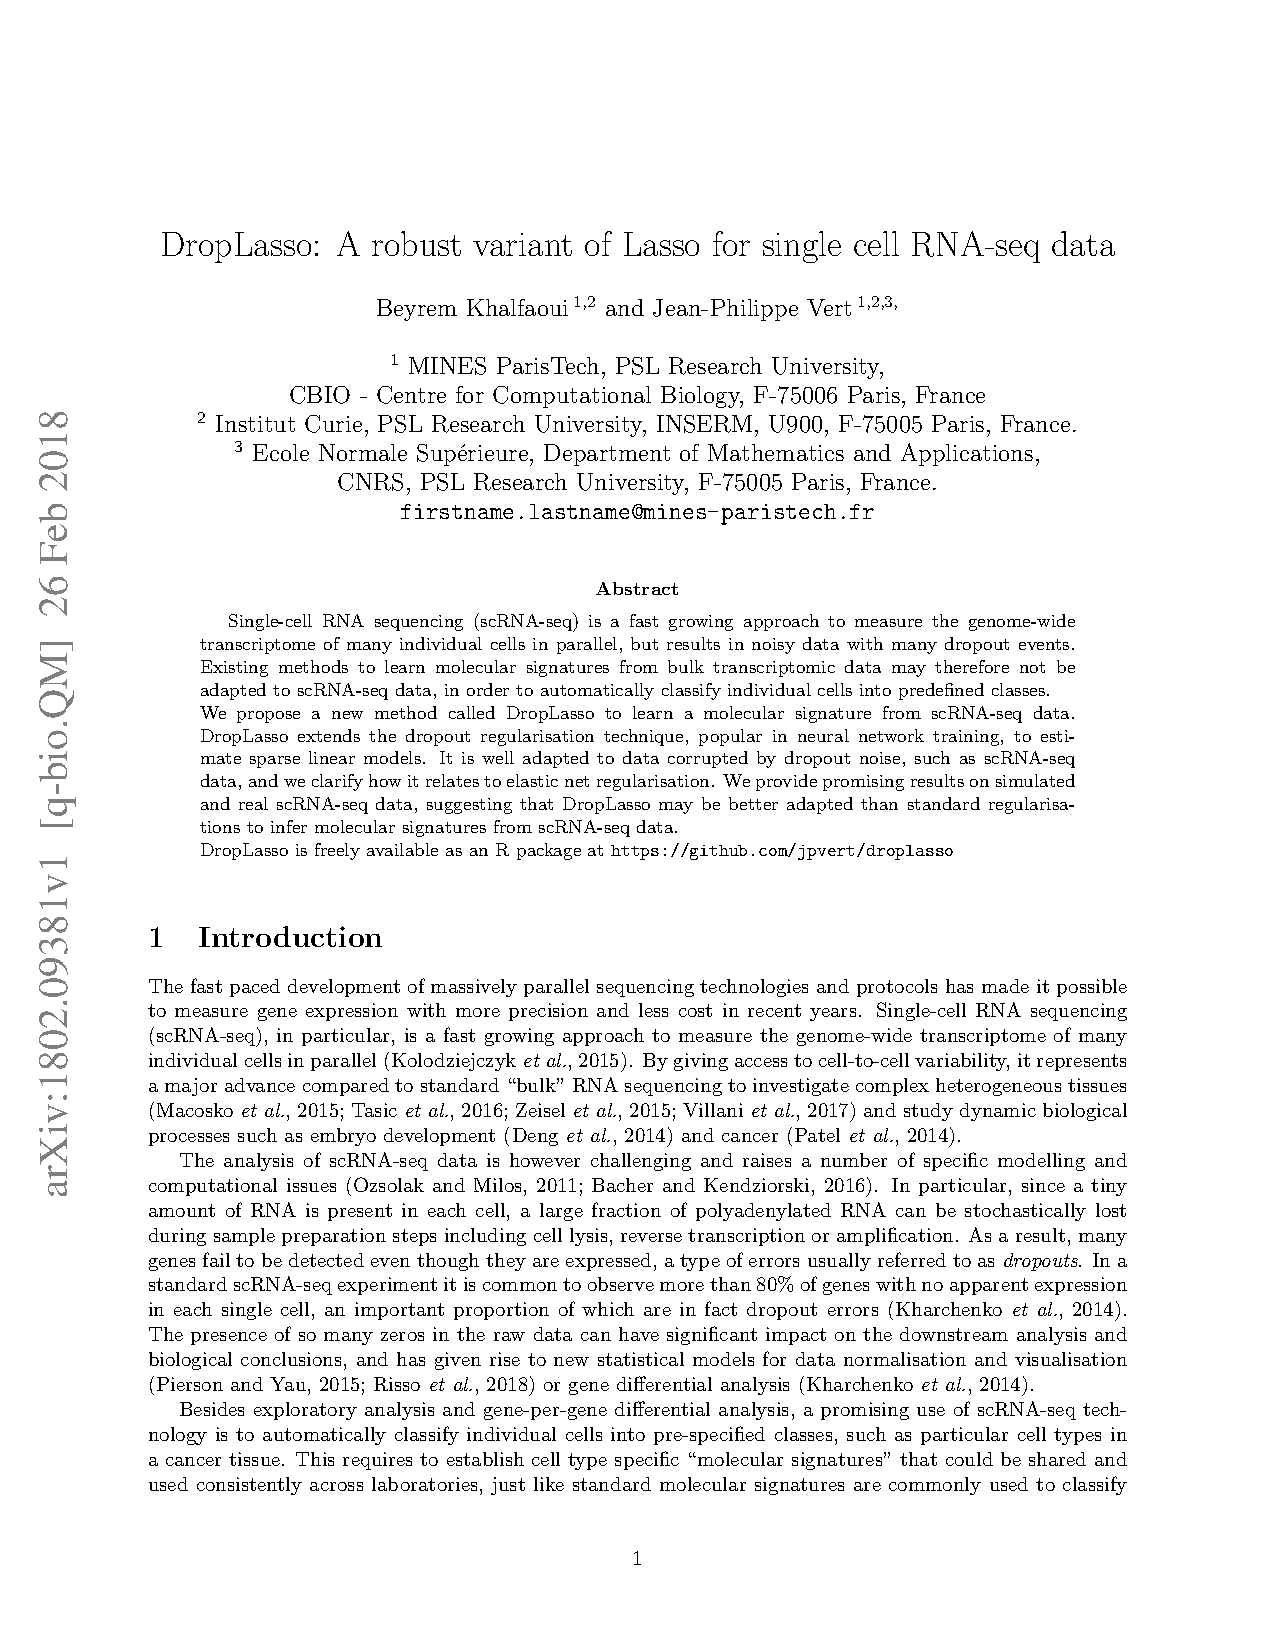
\includegraphics[width=\textwidth]{droplasso}
  \caption{Excerpt from table 3 of ``DropLasso: A robust variant of Lasso for
    single cell RNA-seq data'' Khalfaoui \& Vert (2018)}
\end{figure}

\end{frame}

%%%%%%%%%%%%%%%%%%%%%%%%%%%%%%%%%%%%%%%%%%%%%%%%%%%%%%%%%%%%%%%%%%%%%%%%%%%%%%%%
\section{Conclusions}
\subsection{Comparison}
%%%%%%%%%%%%%%%%%%%%%%%%%%%%%%%%%%%%%%%%%%%%%%%%%%%%%%%%%%%%%%%%%%%%%%%%%%%%%%%%

\begin{frame}{ZINB-WaVE v.~DropLasso}

\begin{itemize}
  \itemsep12pt
  \item ZINB-WaVE is designed to address issues in the statistical analysis
    pipeline that come before differential expression analysis:
    \begin{itemize}
      \item Normalization
      \item Dimensionality Reduction
    \end{itemize}
  \item Since ZINB-WaVE attempts to make scRNA-seq data resemble bulk RNA-seq
    data, the weights can be used with standard differential expression tools.
\end{itemize}

\end{frame}

%%%%%%%%%%%%%%%%%%%%%%%%%%%%%%%%%%%%%%%%%%%%%%%%%%%%%%%%%%%%%%%%%%%%%%%%%%%%%%%%

\begin{frame}{ZINB-WaVE v.~DropLasso}

\begin{itemize}
  \itemsep12pt
  \item DropLasso seeks to cast the scRNA-seq DE problem as a standard Lasso
    problem, accounting for dropout noise using the regularization introduced in
    the neural networks literature.
  \item Since DropLasso is a very new method, there have been no in-depth
    comparisons of the two techniques as of yet.
\end{itemize}

\end{frame}

%%%%%%%%%%%%%%%%%%%%%%%%%%%%%%%%%%%%%%%%%%%%%%%%%%%%%%%%%%%%%%%%%%%%%%%%%%%%%%%%

% don't want dimming with references
\setbeamercovered{}
\beamerdefaultoverlayspecification{}

\begin{frame}[c,allowframebreaks]{References}

\small
\bibliographystyle{plainnat}
\nocite{*}
\bibliography{refs}
\itemize

\end{frame}

%%%%%%%%%%%%%%%%%%%%%%%%%%%%%%%%%%%%%%%%%%%%%%%%%%%%%%%%%%%%%%%%%%%%%%%%%%%%%%%%

\end{document}

